A partir de los datos de en cada figura, encuentra la medida del \'angulo $\angle x^\circ$ para cada una de las siguientes figuras.
%\begin{multicols}{2}

\begin{minipage}[b]{0.42\textwidth}
    \begin{figure}[H]
        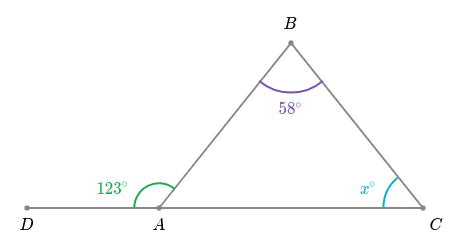
\includegraphics[width=\linewidth]{Images/triangle_angle_01}
        \caption{Diagrama geométrico de un tri\'angulo con base extendida y la inc\'ognita $x$.}
        \label{fig:triangle_angle_01}
    \end{figure}
    \begin{center}
        {\color{cielo}\textbf{$\angle x^\circ =$}} \fbox{
            \begin{minipage}{2cm}
                \hfill\vspace{0.5cm}
            \end{minipage}
        }
    \end{center}
\end{minipage}
\hspace{1cm}
\begin{minipage}[b]{0.42\textwidth}
    \begin{figure}[H]
        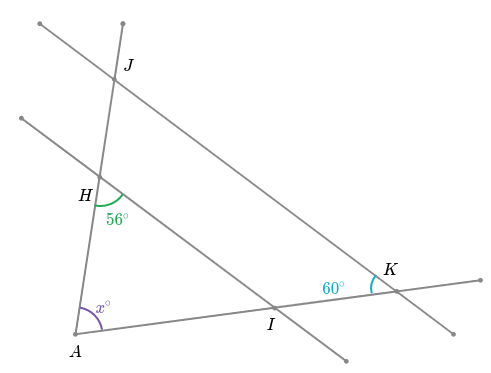
\includegraphics[width=\linewidth]{Images/triangle_angle_04}
        \caption{Diagrama geométrico de la inc\'ognita $x$ con referencia a dos rectas paralelas.}
        \label{fig:triangle_angle_04}
    \end{figure}
    \begin{center}
        {\color{purplePoint}\textbf{$\angle x^\circ =$}} \fbox{
            \begin{minipage}{2cm}
                \hfill\vspace{0.5cm}
            \end{minipage}
        }
    \end{center}

\end{minipage}
%\end{multicols}